\documentclass{beamer}

\usepackage{helvet}
\usepackage{hyperref, graphicx}
\usepackage{amsthm}
\usepackage{etoolbox}
\usepackage{multicol}

\graphicspath{{../../}}

\usetheme{default}
\setbeamertemplate{navigation symbols}{}
\AtBeginSection[ ]
{
\begin{frame}{Outline}
    \tableofcontents[currentsection]
\end{frame}
}

% Default fixed font does not support bold face
\DeclareFixedFont{\ttb}{T1}{txtt}{bx}{n}{11} % for bold
\DeclareFixedFont{\ttm}{T1}{txtt}{m}{n}{12}  % for normal - use in headings

% Custom colors
\usepackage{color}
\definecolor{TUGray}{RGB}{101,101,137}
\definecolor{TUBlack}{RGB}{30,0,0}
\definecolor{mygreen}{RGB}{45,111,63}
\definecolor{keywords}{RGB}{205,114,0}
\definecolor{comments}{RGB}{181,51,139}
\definecolor{strings}{RGB}{58,144,81}
\definecolor{numeric}{RGB}{66,110,176}
\definecolor{linos}{rgb}{0.4,0.4,0.4}
\definecolor{links}{rgb}{0,0.4,0.75}

\definecolor{bggray}{RGB}{232, 233, 235}

\usecolortheme[named=mygreen]{structure}
\setbeamercolor{normal text}{fg=TUBlack}\usebeamercolor*{normal text}

\setbeamercolor{codecol}{fg=TUGray!25!black,bg=bggray}

\hypersetup{colorlinks, linkcolor=links, urlcolor=links}

\usepackage[T1]{fontenc}
\usepackage[sfdefault,scaled=.85]{FiraSans}
\usepackage{newtxsf}

\usepackage{listings}

\newtoggle{InString}{}% Keep track of if we are within a string
\togglefalse{InString}% Assume not initally in string

\newcommand\digitstyle{\color{numeric}}
\makeatletter
\newcommand{\ProcessDigit}[1]
{%
  \ifnum\lst@mode=\lst@Pmode\relax%
   {\digitstyle #1}%
  \else
    #1%
  \fi
}
\makeatother

\lstset{literate=%
    {0}{{{\ProcessDigit{0}}}}1
    {1}{{{\ProcessDigit{1}}}}1
    {2}{{{\ProcessDigit{2}}}}1
    {3}{{{\ProcessDigit{3}}}}1
    {4}{{{\ProcessDigit{4}}}}1
    {5}{{{\ProcessDigit{5}}}}1
    {6}{{{\ProcessDigit{6}}}}1
    {7}{{{\ProcessDigit{7}}}}1
    {8}{{{\ProcessDigit{8}}}}1
    {9}{{{\ProcessDigit{9}}}}1
	{<=}{{\(\leq\)}}1
	{>=}{{\(\geq\)}}1,
	% morestring=[b]",
    % morestring=[b]',
    % morecomment=[l]{//},
}

\lstdefinelanguage{Pseudo}{
    morekeywords={begin, end, return, while},
    morecomment=[l]{\#},
}

% Pseudocode style
\newcommand\pseudostyle{\lstset{
language=Pseudo,
basicstyle=\fontfamily{ccr}\scriptsize,
commentstyle=\it\scriptsize\color{linos},
keywordstyle=\it\bfseries\scriptsize,
mathescape=true,
literate=
    {=}{$\leftarrow{}$}{1}
    {==}{$={}$}{1},
xleftmargin=18pt,
xrightmargin=4pt,
aboveskip=12pt,
belowskip=0pt,
frame=tB,
keepspaces=true
}}

% Python style for highlighting
\newcommand\pythonstyle{\lstset{
language=Python,
basicstyle=\ttfamily\tiny,
numbers=left,
numberstyle=\tiny\color{linos},
morekeywords={self, np},              % Add keywords here
keywordstyle=\tiny\color{keywords},
commentstyle=\it\tiny\color{comments},    % Custom highlighting style
stringstyle=\tiny\color{strings},
xleftmargin=18pt,
xrightmargin=4pt,
aboveskip=0pt,
belowskip=0pt,
escapeinside={(*@}{@*)},
frame=l,                         % Any extra options here
showstringspaces=false,
keepspaces=true
}}

% Pseudocode environment
\lstnewenvironment{pseudo}[1][]
{
    \pseudostyle
    \lstset{
        #1
    }
}
{}

% Python environment 
\lstnewenvironment{python}[1][]
{
	\pythonstyle
	\lstset{
	#1
	}
}
{}

% wrap the Python environment
\newenvironment{codeblock}
    {\hfill\begin{beamerboxesrounded}[lower=codecol, width=0.8\textwidth]
    \medskip

    }
    { 
    \end{beamerboxesrounded}\hfill
    }

\theoremstyle{example}
\newtheorem{question}{Question}

\newcommand{\ct}[1]{\lstinline[language=Python]!#1!}
\newcommand{\ttt}[1]{{\small\texttt{#1}}}
\newcommand{\lsitem}[2]{\ttt{{#1}[}\ct{#2}\ttt{]}}

\author{Chris Cornwell}
\date{Feb 13, 2025}
\title{Assessing accuracy of the LSR line}

\begin{document}

\begin{frame}
\titlepage
\end{frame}

\begin{frame}
\frametitle{Outline}
\tableofcontents
\end{frame}

\section{Assuming the data does have a linear relationship}

%%%%
\begin{frame}
\frametitle{Underlying assumption}
\begin{itemize}
    \item Modeled points in a plane as being from a line, but with noise in the $y$-coordinate direction. In other words, we assumed an underlying relationship 
        \[y = mx + b + \varepsilon\]
    for some $m$ and $b$, and a random variable $\varepsilon$\footnote{$\varepsilon$ is called the error term.} that has expected value 0. Alternatively, among the ``entire population'' there is an LSR line $mx+b$. 
    \pause
    \item Assumption: $\varepsilon$ is independent of $x$.
\end{itemize}

When we have a data set $(x_1,y_1), (x_2,y_2), \ldots, (x_n,y_n)$, from the population, our procedure determines an LSR line $\hat{m}x + \hat{b}$. However, $\hat{m}$ and $\hat{b}$ are not the slope and intercept for the population curve $m$ and $b$.

\end{frame}

%%%%
\begin{frame}[fragile]
\frametitle{Example}
Simulate noisy linear data: make 30 points, using a standard deviation $\sigma = 0.5$. We'll use slope $-1.6$ and intercept $0.8$.
\pause

\begin{codeblock}

\begin{python}
x = np.random.uniform(0, 2, size=30)

def simulate_data(x, std):
    return -1.6*x + 0.8 + np.random.normal(0, std, size=len(x))
y = simulate_data(x, 0.5)
\end{python}

\end{codeblock}

\pause
In groups, compute slope and intercept of the LSR line for a size 30 simulated data set; store $\hat{m}$ and $\hat{b}$ (in two lists). Iterate this 1000 times $\to$ a list of 1000 slopes and intercepts. 

\pause
What is the mean of the slopes and of the intercepts?

\end{frame}

%%%%
\begin{frame}
\frametitle{Sample statistic, relation to population statistic}
This is fundamental to statistics. 
\begin{itemize}
    \item Say that a sample of 2000 people are selected from around the country and their height is measured. Mean of these 2000 heights: sample mean.
    \pause
    \item Sample mean differs from the true mean height of the entire population of the country. (Not by much, perhaps.)
    \begin{itemize}
        \item Weak Law of Large Numbers: if $s$ random samples of 2000 people taken, and each sample mean calculated, as $s\to\infty$, mean of the sample means limits (in probability) to population mean.
    \end{itemize}
    \pause
    \item Analogous thing happens with data from linear relationship with noise {--} think of parameters $\hat{m}$ and $\hat{b}$ as sample statistics (like sample mean).
\end{itemize}

\end{frame}

%%%%
\begin{frame}
\frametitle{Confidence intervals}
How close do we suspect $\hat{m}$ and $\hat{b}$ to be to the ``true'' (population) slope and intercept?

\pause
\textbf{Standard error (SE):}  Suppose that for our error term $\varepsilon$, we have $\operatorname{Var}(\varepsilon) = \sigma^2$. Sample size: $n$.

\pause
Using $\bar{x}$ for the average of $x_1,\ldots,x_n$,

\[SE(\hat{m})^2 = \frac{\sigma^2}{\sum_{i=1}^n(x_i - \bar{x})^2};\]
\[SE(\hat{b})^2 = \sigma^2\left(\frac1{n} + \frac{\bar{x}^2}{\sum_{i=1}^n(x_i - \bar{x})^2}\right).\]

\pause
\emph{Roughly}, these are the amount, on average, that $\hat{m}$ (resp.\ $\hat{b}$) differs from true slope $m$ (resp.\ true intercept $b$).

\pause
$\sigma$ is unknown, but can estimate it with \textbf{residual standard error}:
    \[\hat{\sigma}^2 = RSE^2 = \frac{\sum_{i=1}^n(y_i - \hat{y}_i)^2}{n-2}.\]

\end{frame}


%%%%
\begin{frame}
    \frametitle{Confidence intervals}
    How close do we suspect $\hat{m}$ and $\hat{b}$ to be to the ``true'' (population) slope and intercept?
    
    Formulae: 
    \[SE(\hat{m})^2 = \frac{\sigma^2}{\sum_{i=1}^n(x_i - \bar{x})^2};\]
    \[SE(\hat{b})^2 = \sigma^2\left(\frac1{n} + \frac{\bar{x}^2}{\sum_{i=1}^n(x_i - \bar{x})^2}\right).\]
    
    Estimate:
        \[\sigma^2 \approx RSE^2 = \frac{\sum_{i=1}^n(y_i - \hat{y}_i)^2}{n-2}.\]
    
        \pause
    Can get (roughly) 95\% confidence interval\footnote{95\% of the time, these intervals contain $m$, $b$.} with $\pm 2SE$: 
        \[(\hat{m} - 2SE(\hat{m}), \hat{m} + 2SE(\hat{m}))\]
    and 
        \[(\hat{b} - 2SE(\hat{b}), \hat{b} + 2SE(\hat{b})).\]
    
\end{frame}

\section{Measuring how well LSR line fits}

%%%%
\begin{frame}
\frametitle{Mean Squared Error}
How to measure how well the data fits to regression line?

\pause 
In linear regression, we found $\hat{y}_i, 1\le i\le n$ so that the points $(x_1,\hat{y}_1), \ldots, (x_n, \hat{y}_n)$ fit exactly to a line. Could use average of $(y_i - \hat{y}_i)^2$ as our measure.
    \[ \frac{1}{n}\sum_{i=1}^n (y_i - \hat{y}_i)^2. \]
\pause
\begin{itemize}
    \item Called the mean squared error, MSE, of the LSR line.
    \item Larger MSE (for same sample size), the farther $y_i$ is from $\hat{y}_i$, on average.
\end{itemize}

\pause
Closely related to RSE (residual standard error). Recall, 
    \[\textsf{RSE} = \sqrt{\frac{1}{n-2}\sum_{i=1}^n(y_i - \hat{y}_i)^2}.\]
So $\textsf{MSE} = \frac{n-2}{n}\textsf{RSE}^2$.
\end{frame}

%%%%
\begin{frame}
    \frametitle{Mean Squared Error, example}
    Recall, \lstinline[language=Python, stringstyle=\ttfamily\color{strings}]{'Example1.csv'} data. Its LSR line is 
        \[y = 1.520275x - 0.33458.\]
    \onslide<2->{
    The MSE for this data and its LSR line is $\approx 0.0197$. 

    Does that mean that the linear model is a ``good fit''?
    }

    \vfill
    \centering
    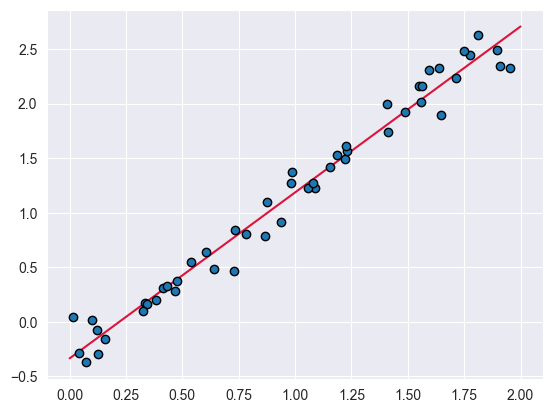
\includegraphics[height=0.35\textheight]{./Lecture04-LinearRegression_1/source/example1-lsrline.png}
\end{frame}

%%%%
\begin{frame}
    \frametitle{Mean Squared Error, scaling}
    What about the following data and its LSR line? Here, the MSE is 1.9746.
    
    \begin{center}
    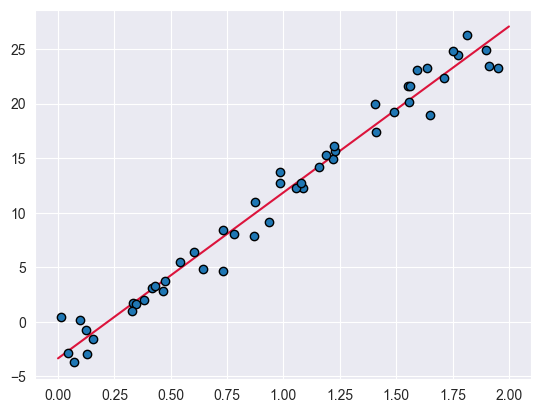
\includegraphics[height=0.35\textheight]{./Images/example1-lsr-scaled.png}    
    \end{center}
    
    Is it still a good fit? 

    \pause
    The data here is from \lstinline[language=Python, stringstyle=\ttfamily\color{strings}]{'Example1.csv'} again, except that the $y$-coordinates have been multiplied by 10. Its LSR line is 
        \[y = 15.20275x - 3.3458.\]
    
    \pause 
    MSE is still a good measure to think about, but its size depends on scale of $y$-coordinates (equivalently, depends on units $y$ is measured in).

\end{frame}

%%%%
\begin{frame}
    \frametitle{$R^2$: Proportion of ``variance explained''}
    Get a measure that is unchanged by scaling: first, set \textbf{total sum of squares} (TSS) to 
    \[\textsf{TSS} = \sum_{i=1}^n(y_i - \bar{y})^2,\]
    where $\bar{y} = \frac{1}{n}\sum_{i=1}^n y_i$.

    \pause 
    Then, 
        \[R^2 = \frac{\textsf{TSS} - n\textsf{MSE}}{\textsf{TSS}} = 1 - \frac{\sum_{i=1}^n(y_i - \hat{y}_i)^2}{\sum_{i=1}^n(y_i - \bar{y}_i)^2}.\]
    \pause
    \begin{itemize}
        \item $R^2$ does \emph{not} depend on the scale of the $y$-coordinates.
        \pause
        \item Any data set, have $0\le R^2\le 1$ (provided $R^2$ is defined; i.e., we do not have $y_1,y_2,\ldots,y_n$ all the same).
        \begin{itemize}
            \item Can you prove this?
        \end{itemize}
    \end{itemize}
\end{frame}

\end{document}